\documentclass{beamer}
\usepackage{etex}
\usepackage{graphicx}
\usepackage[export]{adjustbox}
\usepackage{todonotes}
\usepackage{subcaption}
\usepackage{alltt}
\renewcommand{\ttdefault}{txtt}
\usepackage{ stmaryrd  }
\usepackage{ amssymb }
\usepackage{lmodern}
\usepackage{amsmath}
\newcommand*\rot{\rotatebox{45}}
\usepackage{tikz}
\usetikzlibrary{shapes,arrows,calc,positioning}
\newcommand{\tikzmark}[1]{\tikz[overlay,remember picture] \node (#1) {};}
\usepackage{multicol}
\usepackage{listings}
\usepackage{array}
\usepackage{fancyvrb}
\definecolor{lightgray}{rgb}{.9,.9,.9}
\definecolor{darkgray}{rgb}{.4,.4,.4}
\definecolor{purple}{rgb}{0.65, 0.12, 0.82}
\lstset{
  frame=none,
  xleftmargin=2pt,
  stepnumber=1,
  numbers=left,
  numbersep=5pt,
  numberstyle=\ttfamily\tiny\color[gray]{0.3},
  belowcaptionskip=\bigskipamount,
  captionpos=b,
  escapeinside={*'}{'*},
  language=haskell,
  tabsize=2,
  emphstyle={\bf},
  commentstyle=\it,
  stringstyle=\mdseries\rmfamily,
  showspaces=false,
  keywordstyle=\bfseries\rmfamily,
  columns=flexible,
  basicstyle=\tiny\sffamily,
  showstringspaces=false,
  morecomment=[l]\%,
}
%
% Choose how your presentation looks.
%
% For more themes, color themes and font themes, see:
% http://deic.uab.es/~iblanes/beamer_gallery/index_by_theme.html
%
\mode<presentation>
{
  \usetheme{default}      % or try Darmstadt, Madrid, Warsaw, ...
  \usecolortheme{whale} % or try albatross, beaver, crane, ...
  \usefonttheme{default}  % or try serif, structurebold, ...
  \setbeamertemplate{navigation symbols}{}
  \setbeamertemplate{caption}[numbered]
  \setbeamertemplate{footline}[page number]
  \setbeamercolor{block body}{bg=blue!10,fg=black}
   \setbeamercolor{block title}{bg=structure.fg, fg=white}
  %\addtobeamertemplate{block begin}{\setlength\abovedisplayskip{0pt}}
}

\usepackage[english]{babel}
\usepackage[utf8x]{inputenc}
\captionsetup{compatibility=false}

\title[SYMBOLIC TOPHAT]{A symbolic execution semantics for TopHat}
\author{Nico Naus}
\institute{
\includegraphics[height=3cm,valign=t]{img/uulogo.png}}
\date{September 25th, 2019}

\begin{document}

\begin{frame}
  \titlepage
\end{frame}

% Uncomment these lines for an automatically generated outline.
%\begin{frame}{Outline}
%  \tableofcontents
%\end{frame}

%===================================================
%   INTRODUCTION
%===================================================
\section{Introduction}



\section{Introduction}
\begin{frame}{}

\end{frame}


%===================================================
%  EXAMPLE/MOTIVATION
%===================================================

\section{Example}
\begin{frame}{}

\includegraphics[height=3cm]{img/belastingdienst.png}\\
\pause
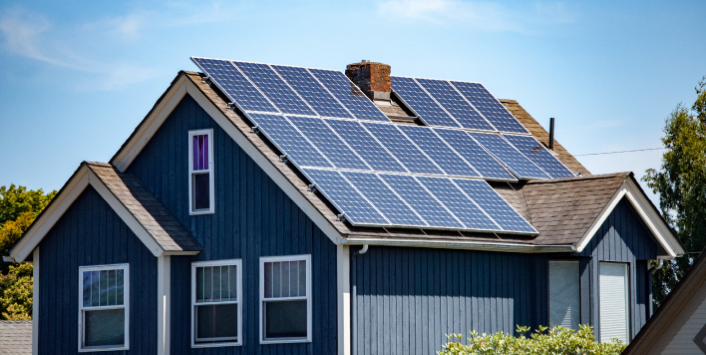
\includegraphics[height=3cm]{img/solar.png}
\end{frame}

%===================================================
%  SYMBOLIC TOPHAT
%===================================================


%===================================================
%  RESULTS
%===================================================


%===================================================
%  OUTLOOK
%===================================================




%===================================================
%  CONCLUSION
%===================================================
\section{Conclusion}


\begin{frame}

\end{frame}

%===================================================
%  APPENDIX
%===================================================
\section*{Appendix}
\appendix

\end{document}
